% Bayes C_mean
\begin{figure}[h]
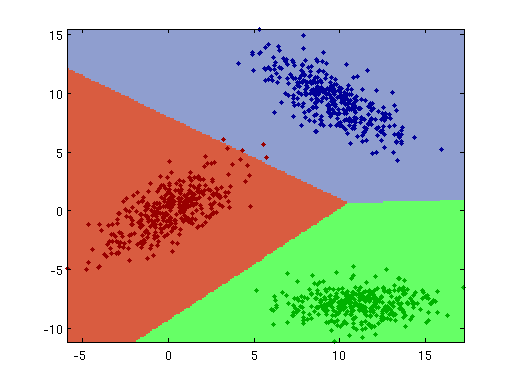
\includegraphics[clip, trim=40px 15px 30px 10px]{data1a_1a.png}
\caption{Bayes $C_{mean}$, Linearly separable data set}}
\end{figure}

\begin{figure}[h]
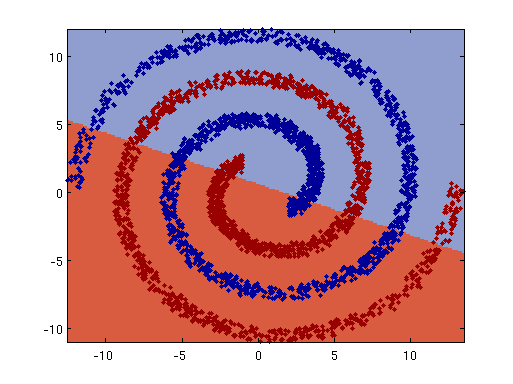
\includegraphics[clip, trim=40px 15px 30px 10px]{data1b_1a.png}
\caption{Bayes $C_{mean}$, Nonlinearly separable data set}
\end{figure}

\begin{figure}[h]
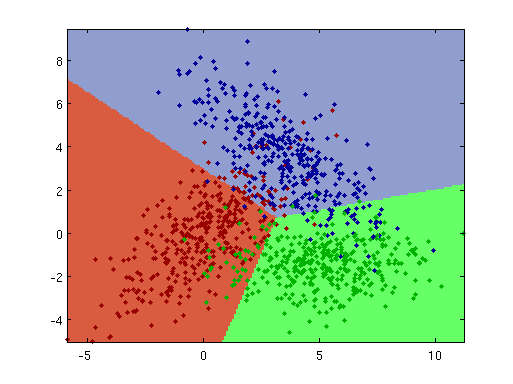
\includegraphics[clip, trim=40px 15px 30px 10px]{data1c_1a.png}
\caption{Bayes $C_{mean}$, Overlapping data set}
\end{figure}

\begin{figure}[h]
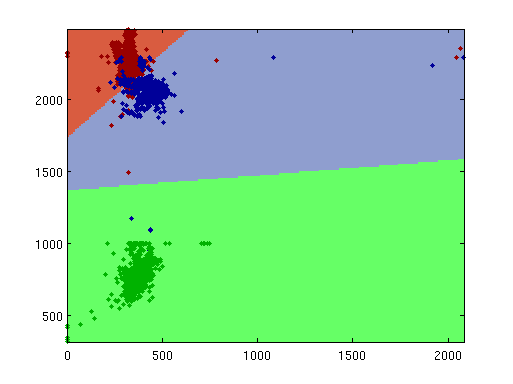
\includegraphics[clip, trim=40px 15px 30px 10px]{data2_1a.png}
\caption{Bayes $C_{mean}$, Real world data set}
\end{figure}



% Bayes C_distinct
\begin{figure}[h]
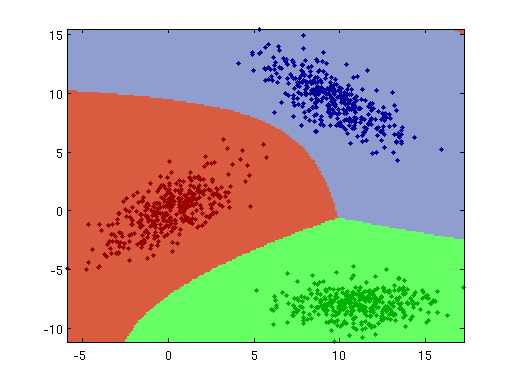
\includegraphics[clip, trim=40px 15px 30px 10px]{data1a_1b.png}
\caption{Bayes $C_{distinct}$, Linearly separable data set}
\end{figure}

\begin{figure}[h]
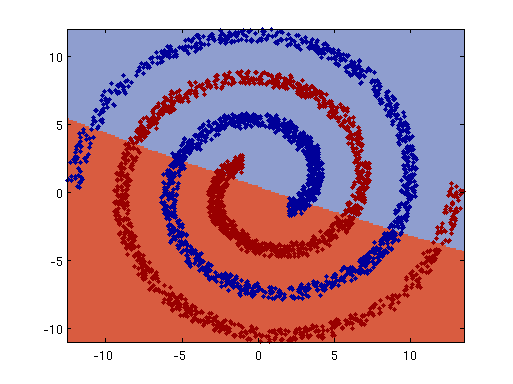
\includegraphics[clip, trim=40px 15px 30px 10px]{data1b_1b.png}
\caption{Bayes $C_{distinct}$, Nonlinearly separable data set}
\end{figure}

\begin{figure}[h]
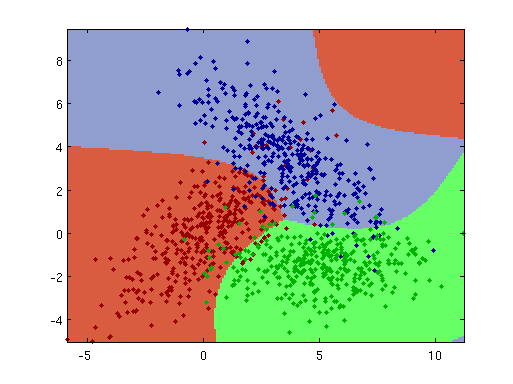
\includegraphics[clip, trim=40px 15px 30px 10px]{data1c_1b.png}
\caption{Bayes $C_{distinct}$, Overlapping data set}
\end{figure}

\begin{figure}[h]
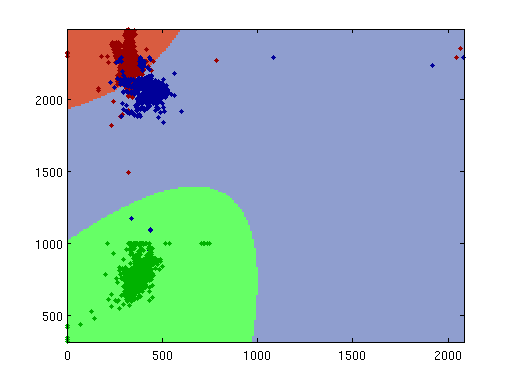
\includegraphics[clip, trim=40px 15px 30px 10px]{data2_1b.png}
\caption{Bayes $C_{distinct}$, Real world data set}
\end{figure}



% Naive Bayes C=\sigma^2 I
\begin{figure}[h]
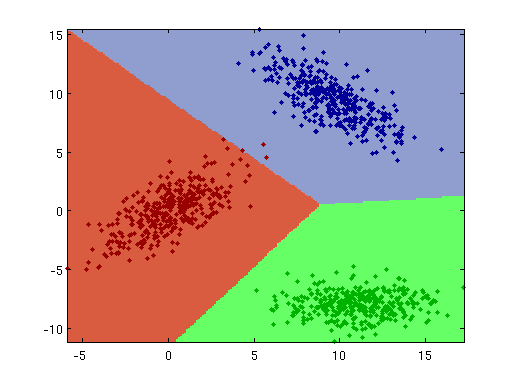
\includegraphics[clip, trim=40px 15px 30px 10px]{data1a_2a.png}
\caption{Naive Bayes $C = \sigma^2 I$, Linearly separable data set}
\end{figure}

\begin{figure}[h]
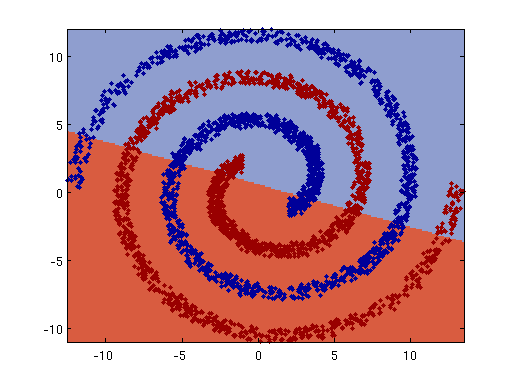
\includegraphics[clip, trim=40px 15px 30px 10px]{data1b_2a.png}
\caption{Naive Bayes $C = \sigma^2 I$, Nonlinearly separable data set}
\end{figure}

\begin{figure}[h]
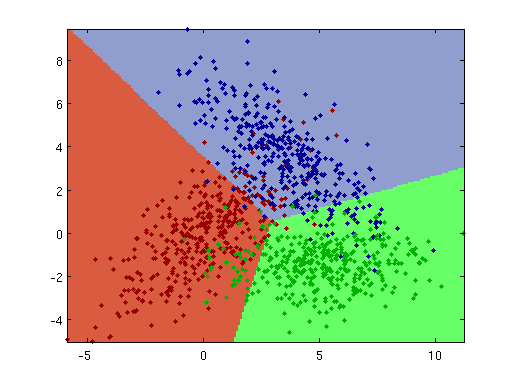
\includegraphics[clip, trim=40px 15px 30px 10px]{data1c_2a.png}
\caption{Naive Bayes $C = \sigma^2 I$, Overlapping data set}
\end{figure}

\begin{figure}[h]
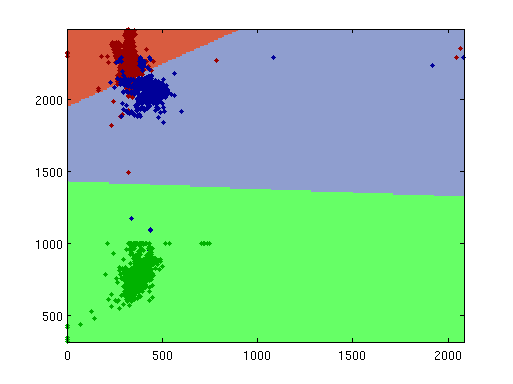
\includegraphics[clip, trim=40px 15px 30px 10px]{data2_2a.png}
\caption{Naive Bayes $C = \sigma^2 I$, Real world data set}
\end{figure}



% Naive Bayes C_mean
\begin{figure}[h]
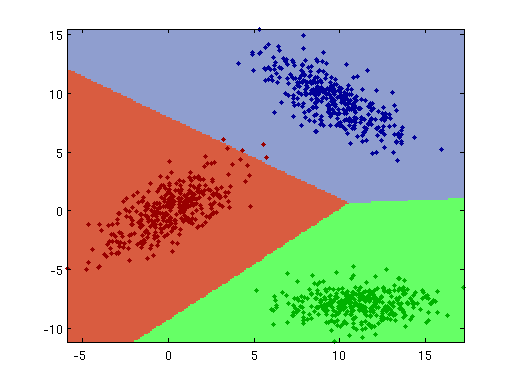
\includegraphics[clip, trim=40px 15px 30px 10px]{data1a_2b.png}
\caption{Naive Bayes $C_{mean}$, Linearly separable data set}
\end{figure}

\begin{figure}[h]
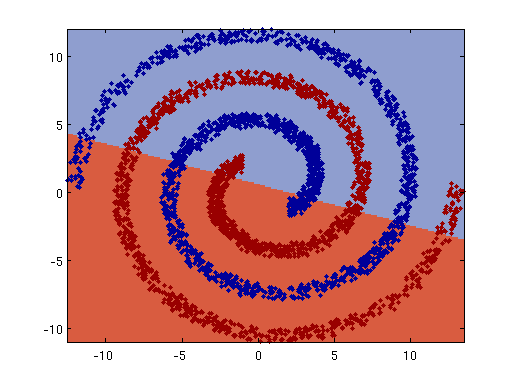
\includegraphics[clip, trim=40px 15px 30px 10px]{data1b_2b.png}
\caption{Naive Bayes $C_{mean}$, Noninearly separable data set}
\end{figure}

\begin{figure}[h]
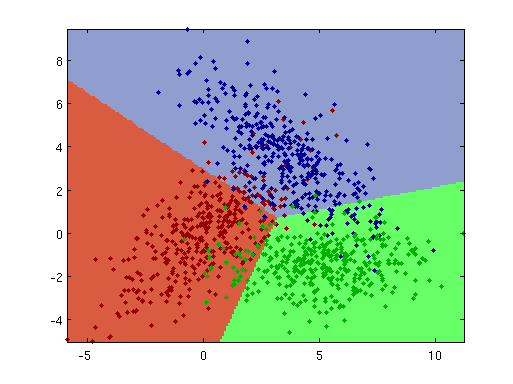
\includegraphics[clip, trim=40px 15px 30px 10px]{data1c_2b.png}
\caption{Naive Bayes $C_{mean}$, Overlapping data set}
\end{figure}

\begin{figure}[h]
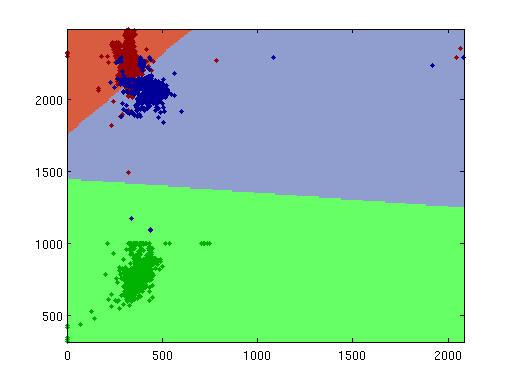
\includegraphics[clip, trim=40px 15px 30px 10px]{data2_2b.png}
\caption{Naive Bayes $C_{mean}$, Real world data set}
\end{figure}



% Naive Bayes C_distinct
\begin{figure}[h]
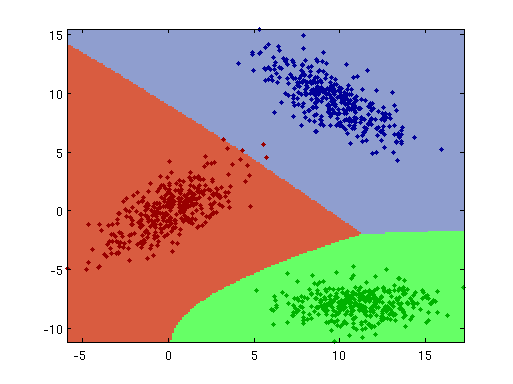
\includegraphics[clip, trim=40px 15px 30px 10px]{data1a_2c.png}
\caption{Naive Bayes $C_{distinct}$, Linearly separable data set}
\end{figure}

\begin{figure}[h]
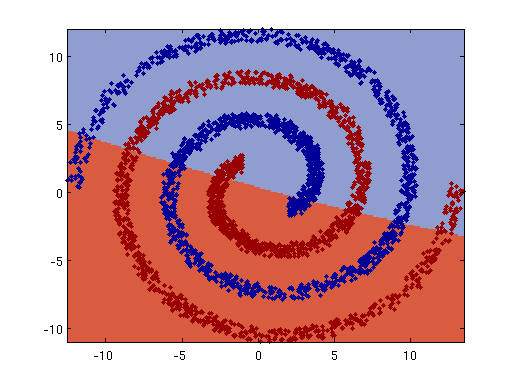
\includegraphics[clip, trim=40px 15px 30px 10px]{data1b_2c.png}
\caption{Naive Bayes $C_{distinct}$, Nonlinearly separable data set}
\end{figure}

\begin{figure}[h]
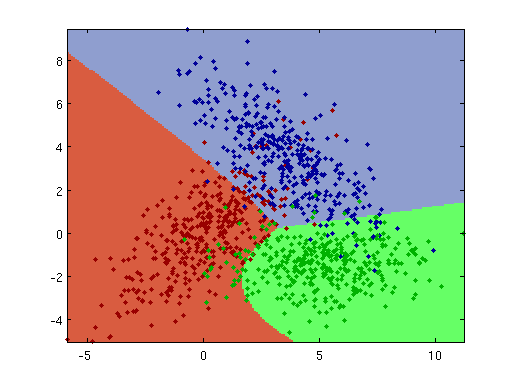
\includegraphics[clip, trim=40px 15px 30px 10px]{data1c_2c.png}
\caption{Naive Bayes $C_{distinct}$, Overlapping data set}
\end{figure}

\begin{figure}[h]
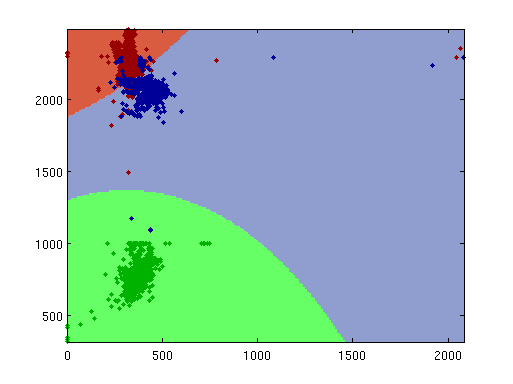
\includegraphics[clip, trim=40px 15px 30px 10px]{data2_2c.png}
\caption{Naive Bayes $C_{distinct}$, Real world data set}
\end{figure}

